\begin{figure}[!h]
  \captionsetup{justification=centering}
  \centering
   

\tikzset{every picture/.style={line width=0.75pt}} %set default line width to 0.75pt        

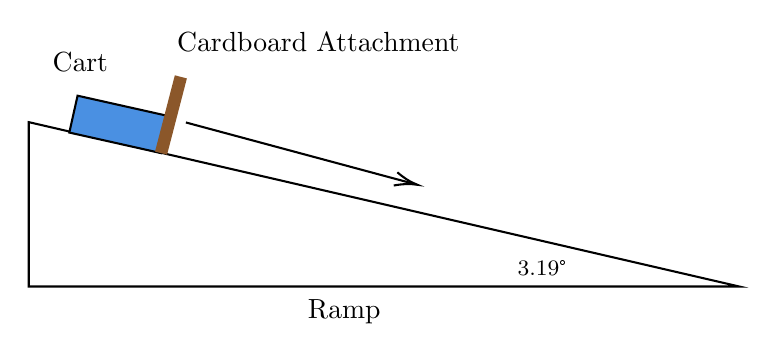
\begin{tikzpicture}[x=0.75pt,y=0.75pt,yscale=-1,xscale=1]
%uncomment if require: \path (0,300); %set diagram left start at 0, and has height of 300

%Shape: Right Triangle [id:dp18569224305294485] 
\draw   (3,189) -- (345.3,268.2) -- (3,268.2) -- cycle ;
%Shape: Rectangle [id:dp7438562411637597] 
\draw  [fill={rgb, 255:red, 74; green, 144; blue, 226 }  ,fill opacity=1 ] (26.54,176.27) -- (70.74,186.17) -- (66.76,203.93) -- (22.56,194.03) -- cycle ;
%Straight Lines [id:da735201395514776] 
\draw [color={rgb, 255:red, 139; green, 87; blue, 42 }  ,draw opacity=1 ][line width=4.5]    (76.3,167.2) -- (66.76,203.93) ;
%Straight Lines [id:da10025482914979356] 
\draw    (78.74,189.17) -- (188.37,218.68) ;
\draw [shift={(190.3,219.2)}, rotate = 195.06] [color={rgb, 255:red, 0; green, 0; blue, 0 }  ][line width=0.75]    (10.93,-3.29) .. controls (6.95,-1.4) and (3.31,-0.3) .. (0,0) .. controls (3.31,0.3) and (6.95,1.4) .. (10.93,3.29)   ;

% Text Node
\draw (237,254) node [anchor=north west][inner sep=0.75pt]   [align=left] {{\fontfamily{}\selectfont {\footnotesize 3.19°}}};
% Text Node
\draw (13,154) node [anchor=north west][inner sep=0.75pt]   [align=left] {{\fontfamily{}\selectfont Cart}};
% Text Node
\draw (73,144) node [anchor=north west][inner sep=0.75pt]   [align=left] {{\fontfamily{}\selectfont Cardboard Attachment}};
% Text Node
\draw (136,273) node [anchor=north west][inner sep=0.75pt]  [align=left] {{\fontfamily{}\selectfont Ramp}};


\end{tikzpicture}
\caption{General experimental setup with a Smart Cart rolling down a ramp. Cross-sectional area of the cart is changed using a cardboard attachment.}
\label{fig:basicramp}
\end{figure}

Figure \ref{fig:basicramp} shows the basic experimental configuration of this experiment. The cart was rolled down
a ramp with an attachment on its front. Said attachment modified the cart's cross-sectional area as well as its
aerodynamic properties. 

We can break down the forces experienced by the cart into components \ref{fig:basicramp} as shown in the free body diagram below.

\begin{figure}[!h]
  \captionsetup{justification=centering}
  \centering
\tikzset{every picture/.style={line width=0.75pt}} %set default line width to 0.75pt        

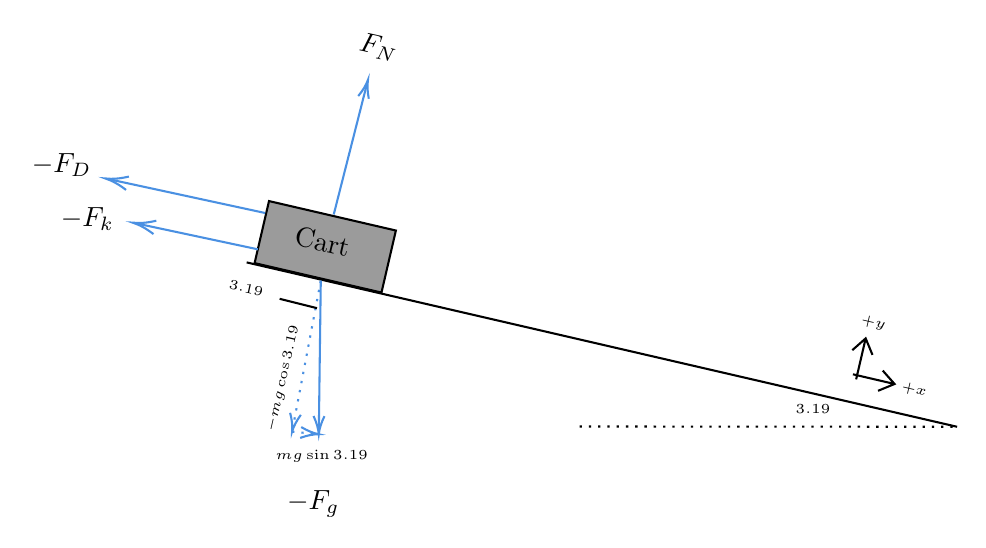
\begin{tikzpicture}[x=0.75pt,y=0.75pt,yscale=-1,xscale=1]
%uncomment if require: \path (0,300); %set diagram left start at 0, and has height of 300

%Straight Lines [id:da25597455715040285] 
\draw    (159,125.8) -- (501.3,205) ;
%Shape: Rectangle [id:dp8095676769699147] 
\draw  [fill={rgb, 255:red, 155; green, 155; blue, 155 }  ,fill opacity=1 ] (169.77,96.25) -- (230.9,110.44) -- (223.96,140.33) -- (162.83,126.14) -- cycle ;
%Straight Lines [id:da9581258174951208] 
\draw [color={rgb, 255:red, 74; green, 144; blue, 226 }  ,draw opacity=1 ]   (200.96,102.71) -- (216.97,39.77) ;
\draw [shift={(217.46,37.83)}, rotate = 464.27] [color={rgb, 255:red, 74; green, 144; blue, 226 }  ,draw opacity=1 ][line width=0.75]    (8.74,-2.63) .. controls (5.56,-1.12) and (2.65,-0.24) .. (0,0) .. controls (2.65,0.24) and (5.56,1.12) .. (8.74,2.63)   ;
%Straight Lines [id:da5736220263506606] 
\draw [color={rgb, 255:red, 74; green, 144; blue, 226 }  ,draw opacity=1 ]   (194.72,134.63) -- (193.78,206.58) ;
\draw [shift={(193.75,208.58)}, rotate = 270.75] [color={rgb, 255:red, 74; green, 144; blue, 226 }  ,draw opacity=1 ][line width=0.75]    (8.74,-2.63) .. controls (5.56,-1.12) and (2.65,-0.24) .. (0,0) .. controls (2.65,0.24) and (5.56,1.12) .. (8.74,2.63)   ;
%Straight Lines [id:da19213091912892] 
\draw [color={rgb, 255:red, 74; green, 144; blue, 226 }  ,draw opacity=1 ] [dash pattern={on 0.84pt off 2.51pt}]  (194.72,134.63) -- (181.27,205.39) ;
\draw [shift={(180.9,207.35)}, rotate = 280.76] [color={rgb, 255:red, 74; green, 144; blue, 226 }  ,draw opacity=1 ][line width=0.75]    (8.74,-2.63) .. controls (5.56,-1.12) and (2.65,-0.24) .. (0,0) .. controls (2.65,0.24) and (5.56,1.12) .. (8.74,2.63)   ;
%Straight Lines [id:da7747687861398798] 
\draw [color={rgb, 255:red, 74; green, 144; blue, 226 }  ,draw opacity=1 ] [dash pattern={on 0.84pt off 2.51pt}]  (180.9,207.35) -- (191.76,208.39) ;
\draw [shift={(193.75,208.58)}, rotate = 185.46] [color={rgb, 255:red, 74; green, 144; blue, 226 }  ,draw opacity=1 ][line width=0.75]    (8.74,-2.63) .. controls (5.56,-1.12) and (2.65,-0.24) .. (0,0) .. controls (2.65,0.24) and (5.56,1.12) .. (8.74,2.63)   ;
%Straight Lines [id:da9726247084266131] 
\draw    (174.9,143.35) -- (192.9,147.85) ;
%Straight Lines [id:da06568273382266154] 
\draw  [dash pattern={on 0.84pt off 2.51pt}]  (319.4,204.85) -- (501.3,205) ;
%Straight Lines [id:da2330937848478929] 
\draw [color={rgb, 255:red, 74; green, 144; blue, 226 }  ,draw opacity=1 ]   (167.9,102) -- (92.85,85.77) ;
\draw [shift={(90.9,85.35)}, rotate = 372.2] [color={rgb, 255:red, 74; green, 144; blue, 226 }  ,draw opacity=1 ][line width=0.75]    (10.93,-3.29) .. controls (6.95,-1.4) and (3.31,-0.3) .. (0,0) .. controls (3.31,0.3) and (6.95,1.4) .. (10.93,3.29)   ;
%Shape: Axis 2D [id:dp4847297973478324] 
\draw  (451.1,179.71) -- (471.16,184.38)(457.24,162.41) -- (452.65,182.15) (465.47,177.92) -- (471.16,184.38) -- (463.21,187.66) (450.79,168.1) -- (457.24,162.41) -- (460.53,170.36)  ;
%Straight Lines [id:da11556239096826859] 
\draw [color={rgb, 255:red, 74; green, 144; blue, 226 }  ,draw opacity=1 ]   (164.4,119.5) -- (106.06,107.07) ;
\draw [shift={(104.1,106.65)}, rotate = 372.03] [color={rgb, 255:red, 74; green, 144; blue, 226 }  ,draw opacity=1 ][line width=0.75]    (10.93,-3.29) .. controls (6.95,-1.4) and (3.31,-0.3) .. (0,0) .. controls (3.31,0.3) and (6.95,1.4) .. (10.93,3.29)   ;

% Text Node
\draw (182.5,106.58) node [anchor=north west][inner sep=0.75pt]  [rotate=-13.1] [align=left] {{\fontfamily{}\selectfont Cart}};
% Text Node
\draw (474.25,181.21) node [anchor=north west][inner sep=0.75pt]  [font=\tiny,rotate=-13.1]  {$+x$};
% Text Node
\draw (454.75,149.21) node [anchor=north west][inner sep=0.75pt]  [font=\tiny,rotate=-13.1]  {$+y$};
% Text Node
\draw (213.64,13.21) node [anchor=north west][inner sep=0.75pt]  [rotate=-12.6]  {$F_{N}$};
% Text Node
\draw (54,71.9) node [anchor=north west][inner sep=0.75pt]    {$-F_{D}$};
% Text Node
\draw (150,132.41) node [anchor=north west][inner sep=0.75pt]  [font=\tiny,rotate=-12.8]  {$3.19\degree $};
% Text Node
\draw (177,234.4) node [anchor=north west][inner sep=0.75pt]    {$-F_{g}$};
% Text Node
\draw (422,192.9) node [anchor=north west][inner sep=0.75pt]  [font=\tiny]  {$3.19\degree $};
% Text Node
\draw (171.5,214.9) node [anchor=north west][inner sep=0.75pt]  [font=\tiny]  {$mg\sin 3.19\degree $};
% Text Node
\draw (166,208) node [anchor=north west][inner sep=0.75pt]  [font=\tiny,rotate=-283]  {$-mg\cos 3.19\degree $};
% Text Node
\draw (68,97.9) node [anchor=north west][inner sep=0.75pt]    {$-F_{k}$};


\end{tikzpicture}
\caption{Free body diagram illustrating various forces acting upon the Smart Cart}
\label{fbdcart}
\end{figure}

In the free body diagram in figure \ref{fbdcart}, the cart is on the ramp, with the forces of air resistance ($F_{D}$) and kinetic friction ($F_{k}$) acting
against the cart in the horizontal direction. The cart is also accelerated down the ramp by the horizontal component of gravity ($mg\sin(3.19\degree)$).


\begin{gather*}
  F_{\textup{net}} = mg\sin(\theta) - F_{K} - kv^2\\
  \\
  ma = mg\sin(\theta) - F_{K} - kv^2\\
\end{gather*}
\begin{equation}
  a = \frac{mg\sin(\theta) - F_{K} - kv^2}{m}
  \label{Eq:acceleration} %the label lets you refer to the equation later
\end{equation}


